\section{Funktionale Anforderungen}

\subsection{Programmausführung}
	
	\begin{description}
		
		\item[/F010/] \textit{Programm beenden:}\par Im ganzen Programm die Möglichkeit gegeben, durch betätigen der "`Fenster schließen"' Schaltfläche (differiert je nach Betriebssystem), das Programm zu beenden.
		
		% TODO Schaltfläche benennen
		\item[/F020/] \textit{Speicherverhalten:}\par Nach jedem Dialog, ist die Möglichkeit gegeben, die aktuelle Änderung für die aktuelle Programmausführung zu sichern. Sollen Änderungen dauerhaft gesichert werden, muss die Schaltfläche "`XXX"' betätigt werden. Durch betätigen dieser Schaltfläche, wird die Projektkonfigurationsdatei neu generiert und in dem Projektordner gespeichert.
		
		\item[/F030/] \textit{Automatische Anpassung der Größe der Bedienoberfläche:}\par Das Programm positioniert automatisch seine Bedienelemente, in Abhängigkeit zur Auflösung des Programmfensters.
		
		%TODO Guireferenz
		\item[/F040/] \textit{Automatisches durchsuchen des Projektordners:}\par Bei Programmstart, wird in dem Projektordner des Programms nach Projektkonfigurationsdateien gesucht. Auf der Basis dieser Datensätze wird eine Projektliste generiert, die in einem Dialog, nach absteigendem Bearbeitungsdatum (aktuelles zuerst), sortiert angezeigt werden. Zudem wird das Datum anders formatiert dargestellt als der Projektname. (siehe Kapitel REF)
		
	\end{description}

\subsection{Projektmanagement}

\label{subsec:projektmanagement}
	
	\gls{tempX} verfügt über eine eingebaute Projektverwaltung, mit der der Benutzer beliebige Kombinationen von Bildmengen und Auswertungen verwalten kann. Es kann allerdings immer nur ein Projekt im aktiven Zustand sein, ein Wechsel in ein anderes Projekte während der Programmausführung ist möglich.
	
	\begin{description}		
		
		%TODO Projektordner benennen, GUI
		\item[/F110/] \textit{Neues Projekt anlegen:}\par In dem Dialog aus \textbf{/F040/}, ist die Möglichkeit gegeben, durch betätigen der Schaltfläche "`Projekt erstellen"', ein neues Projekt zu erstellen und ihm einen Namen zu geben.\par Dabei wird überprüft, ob dieser Projektname schon von einem anderen Projekt verwendet wird. Ist dies der Fall, kann der Benutzer einen neuen Namen eingeben. Dabei ist auch zu beachten, dass der Projektname zwischen einem und 255 Zeichen lang sein muss.\par Nun wird eine neue Projektkonfigurationsdatei im PROJEKTE-Ordner angelegt. Bei der Projektanlegung wird auch ein Erstellungsdatum gespeichert (siehe Kapitel \ref{subsec:programmdaten} \textbf{/D20/}). Danach wird das Hauptprogramm gestartet, mit dem gerade erstellten Projekt (siehe Kapitel \ref{subsec:benutzerschnittstelle}).
		
		\item[/F120/] \textit{Projekt aktivieren:}\par Um eine Projekt zu aktivieren, muss man es in der Liste der Projekte, in dem Dialog aus \textbf{/F040/}, auswählen.
		
		%TODO GUI
		\item[/F130/] \textit{Vorhandens Projekt öffnen:}\par In dem Dialog aus \textbf{/F040/}, ist die Möglichkeit gegeben, durch einen Doppelklick, mit der linken Maustaste, auf den Projektnamen eines bereits vorhanden Projektes oder durch aktivieren eines Projektes und betätigen der Schaltfläche "`Projekt öffnen"' (siehe Kapitel \ref{subsec:benutzerschnittstelle}, das Hauptprogramm zu starten.\par In der damit verbundenen Projektkonfigurationsdatei gespeicherte Bildmengen und Auswertungen werden nun verfügbar gemacht. Damit gemeint ist: 
			
			\begin{itemize}
				
				\item Das Einlesen von \gls{exif}-Parametern aller Bilder, die in den Bildmengen des Projekts definiert sind. Das Einlesen geschieht im Hintergrund, d.h. der Benutzer kann mit dem Programm interagieren, vollständige Funktionalität ist aber erst nach dem vollständigen Einlesen der \gls{exif} Daten gegeben.
				
				\item Anzeige der Bildmengen (siehe Kapitel \ref{subsec:bildmengenmgmt} \textbf{/F250/}).
				
				\item Anzeige der Auswertungen (siehe Kapitel \ref{subsec:auswertungsmgmt}).
				
				% TODO in GUI kennzeichnen
				\item Anzeige aller Bilder der Bildmengen in dem Bereich "`Bildansicht"' und aktivieren des ersten Bildes. Dadurch wird der Bildbereich "`\gls{exif}-Daten"' mit den \gls{exif}-Parametern dieses Bildes aktualisiert.
			
			\end{itemize}		
		
		\item[/F140/] \textit{Projekt kopieren:}\par In dem Dialog aus \textbf{/F040/}, ist die Möglichkeit gegeben, ein aktiviertes Projekt mit allen in ihm definierten Daten, Bildmengen und Auswertungen zu kopieren und es unter neuem Namen und neuem Erstellungsdatum abzuspeichern. Danach, wird das Hauptprogramm gestartet, mit dem gerade kopierten Projekt (siehe Kapitel \ref{subsec:benutzerschnittstelle}).
		
		\item[/F150/] \textit{Projekt entfernen:}\par In dem Dialog aus \textbf{/F040/}, ist die Möglichkeit gegeben, bei einem aktivierten Projekt, mit betätigen der Schaltfläche "`Projekt entfernen"', folgende Aktionen auszulösen:
			
			\begin{enumerate}
				
				\item Es wird eine Sicherheitsabfrage (ein Dialog mit Ja/Nein Auswahlmöglichkeit) angezeigt, die dem Benutzer die Möglichkeit gibt, das Entfernen abzubrechen.
				
				\item Das Projekt wird aus der Liste des Dialogs entfernt.
				
				\item Die Projektkonfigurationsdatei, wird in dem Projektordner gelöscht.
				
				\item Dem Benutzer wird eine Rückmeldung gegeben, ob das Entfernen erfolgreich war oder ob es einen Fehler gab.
			
			\end{enumerate}
	
	\end{description}

\subsection{Bildmengenmanagement}

\label{subsec:bildmengenmgmt}
	
	In einem Projekt, können Bildmengen verwaltet werden (siehe Kapitel \ref{sec:nichtfunktionale_anforderungen} \textbf{/NF020/}). Eine Bildmenge ist folgendermaßen definiert:
	
	\begin{itemize}
		
		\item Eine Bildmenge kann ein oder mehrere Verweise auf Bilder (im \gls{jpg}-Format) des verwendeten Dateisystems enthalten.
		
		\item Eine Bildmenge kann ein oder mehrere Verweise auf Ordner des verwendeten Dateisystems enthalten.
		
		\item Eine Bildmenge kann ein oder mehrere Verweise auf Bildmengen haben, die in dem Projekt definiert sind. Dabei ist zu beachten:
		
			\begin{itemize}
			
				\item Bei den Verweisen, darf es zu keinen Endlosverweisen führen (Bildmenge A ist in Bildmenge B und Bildmenge B ist in Bildmenge A).
				
				\item Wird eine Bildmenge entfernt, so wird ein Verweis auf diese Bildmenge ebenfalls entfernt.
			
			\end{itemize}
		
		\item Eine Bildmenge hat einen frei definierbaren und vom Projektkontext abhängigen eindeutigen Namen, der zwischen einem und 255 Zeichen lang sein muss.
		
		\item Eine Bildmenge wird über eine interne ID eindeutig identifiziert.
	
	\end{itemize}
	
	% TODO GUI
	Es ist außerdem zu beachten, dass bei einem Dateisystem- oder einem Datenspeicherstrukturwechsel die Verweise keine Gültigkeit mehr haben können und ein Neuanlegen dieser Verweise unumgänglich ist.\par Wird ein Projekt geöffnet, werden alle in der Projektkonfigurationsdatei definierten Bildmengen \gls{lexgraph} sortiert angezeigt. Die erste Bildmenge der Liste (falls vorhanden), wird dabei automatisch auf aktiv gesetzt (siehe Kapitel GUI).
	
	\begin{description}
		
		\item[/F210/] \textit{Anlegen einer neuen Bildmenge:}\par Durch betätigen der Schaltfläche "`Erstellen"' im Bereich Bildmengen, wird ein Dialog (der je nach verwendetem Betriebssystem eine unterschiedliche Handhabung hat) geöffnet, der dem Benutzer folgende Möglichkeiten gibt:
			
			\begin{itemize}
			
				\item Auswahl ein oder mehrerer Ordner, die einzeln als Pfade zum jeweiligen Ordner in die Bildmenge übernommen werden. Ausgehend von diesen Ordnern, wird rekursiv der Verzeichnisbaum nach Bilder im \gls{jpg}-Format durchsucht.
				
				\item Auswahl ein oder mehrerer Bilder im \gls{jpg}-Format, deren Pfade einzeln in die Bildmenge übernommen werden.
			
			\end{itemize}
		
		Nach dem Durchsuchen, wird ein weiterer Dialog geöffnet, der die Möglichkeit gibt der Bildmenge einen Namen zu geben.
		
		\item[/F220/] \textit{Aktivieren einer Bildmenge:}\par Um eine Bildmenge zu aktivieren, muss man sie in der Liste der Bildmengen, im Bereich "`Bildmengen"', auswählen. Dadurch wird der Bereich "`Inhalt"' aktualisiert (siehe Kapitel \textbf{/F250/}).
		
		\item[/F230/] \textit{Hinzufügen von Bildern und Ordnern zu einer vorhandenen Bildmenge:}\par Um diese Aktionen auszuführen, muss eine Bildmenge aktiv sein. Das Hinzufügen kann über zwei Arten geschehen:
		
			\begin{itemize}
				
				% TODO GUI
				\item Durch \gls{dragndrop} von Ordnern und Bildern aus der grafischen Benutzerschnittstelle des Betriebssystems in den Bereich "`Inhalt"', einer aktiven Bildmenge (siehe Kapitel GUI). 
				
				\item Durch betätigen der Schaltfläche "`Hinzufügen"' in dem Bereich "`Inhalt"' einer aktiven Bildmenge, wird ein Dialog geöffnet, der analog zu dem in Funktion \textbf{/F210/} beschriebenen Dialog arbeitet. Auch die folgenden Schritte sind analog.
			
			\end{itemize}
		
		\item[/F240/] \textit{Hinzufügen von Bildmengen zu einer vorhandenen Bildmenge:}\par Das Hinzufügen kann nur per \gls{dragndrop} einer vorhanden Bildmenge aus dem Bereich "`Bildmengen"' in den Bereich "`Inhalt"' einer aktiven Bildmenge erfolgen. Dabei wird die Definition von Bildmengen eingehalten (siehe Kapitel \ref{subsec:bildmengenmgmt}).
		
		\item[/F250/] \textit{Entfernen von Bildmengen:}\par Um diese Aktionen auszuführen, muss eine Bildmenge aktiv sein. Durch betätigen der Schaltfläsche "`Entfernen"', werden folgende Aktionen ausgelöst:
			
			\begin{enumerate}
			
				\item Es wird eine Sicherheitsabfrage (ein Dialog mit Ja/Nein Auswahlmöglichkeit) angezeigt, die dem Benutzer die Möglichkeit gibt, das Entfernen abzubrechen.
				
				\item Die Bildmenge wird aus der Liste der Bildmengen entfernt.
				
				\item Es werden alle restlichen Bildmengen nach Verweisen auf diese Bildmenge durchsucht. Falls Verweise vorhanden sind, werden diese Verweise entfernt.
				
				\item Dem Benutzer wird eine Rückmeldung gegeben, ob das Entfernen erfolgreich war oder ob es einen Fehler gab.
				
				\item Nach dem Entfernen, ist die erste Bildmenge (falls vorhanden) in der Liste aktiv.
			
			\end{enumerate}

		\item[/F260/] \textit{Aufbau der Inhaltsliste:}\par Ist eine Bildmenge aktiv, wie in dem Bereich "`Inhalt"' die Liste mit dem Inhalt der Bildmenge aktualisiert. Die Liste wird dabei blockweise nach folgendem Schema aufgebaut:
		
			\begin{enumerate}
			
				\item Mit der Bildmenge verknüpfte Bildmengen, \gls{lexgraph} sortiert.
			
				\item Mit der Bildmenge verknüpfte Verweise auf Ordner, \gls{lexgraph} sortiert.
				
				\item Mit der Bildmenge verknüpfte Verweise auf Bilder, \gls{lexgraph} sortiert.
				
			\end{enumerate}
			
			Jeder Block ist dabei mit einer unterschiedlichen Textfarbe formatiert.
		
	\end{description}

\subsection{Diagrammmanagement}

\label{subsec:diagrammmgmt}

	\gls{tempX} beherrscht verschiedene Diagrammtypen, welche im folgenden genannt sind:
	
	\begin{description}

		\item[/F310/] \textit{Tabelle:}\par 
		
			\begin{figure}[H]
				\centering
				\fbox{
					\begin{minipage}{13 cm}
						\centering
						\resizebox{13 cm}{!} {
\begin{tabular}{|c|c|c|c|c|c|c|}
\hline  Name & Manufacturer & Date and Time & FNumber & Exposure Time & Flash \\ 
\hline  DSC00601.JPG & Sony Ericsson   & 2009:11:07 00:27:48  & f/2,8 & 1/1000 & False\\ 
\hline  DSC00602.JPG & Sony Ericsson & 2009:11:06 10:27:26 & f/2,8  & 1/1600 & False \\ 
\hline  DSC00606.JPG & Sony Ericsson & 2009:11:06 12:35:59 & f/2,8  & 1/800 & False \\ 
\hline  SDC16734.JPG & Samsung Techwin & 2009:11:05 00:59:01   & f/7,0 & 1/250 & False\\ 
\hline  SDC16742.JPG & Samsung Techwin & 2009:11:06 05:52:36   & f/7,1 & 1/250 & False\\ 
\hline 
\end{tabular} 

}
						\caption{Ansicht einer tabellarischen Auswertung}
						\label{diag:tabelle}
					\end{minipage}  
				}    		
			\end{figure}			
			Die Tabelle stellt alle auszuwertenden \gls{exif}-Daten mit Dateinamen tabellarisch dar (siehe Kapitel \ref{subsec:auszuwertendedaten}). Dabei wird absteigend nach dem Dateinamen sortiert. Die Tabelle kann als \gls{jpg} exportiert werden.

		\item[/F320/] \textit{2D Histogramm:}\par 
		
			\begin{figure}[H]
				\centering
				\fbox{
					\begin{minipage}{13 cm}
						\centering						
						% Generated with LaTeXDraw 2.0.2
% Tue Nov 17 17:42:28 CET 2009
% \usepackage[usenames,dvipsnames]{pstricks}
% \usepackage{epsfig}
% \usepackage{pst-grad} % For gradients
% \usepackage{pst-plot} % For axes
\scalebox{1} % Change this value to rescale the drawing.
{
\begin{pspicture}(0,-3.6579165)(12.652083,3.6979167)
\definecolor{color2405b}{rgb}{0.3764705882352941,0.6666666666666666,0.9921568627450981}
\rput(0.74583334,-2.9120834){\psaxes[linewidth=0.04,ticksize=0.10583333cm,dx=1.15cm,dy=1.0cm,Dx=100]{->}(0,0)(0,0)(11,6)}
\psframe[linewidth=0.04,dimen=outer,fillstyle=solid,fillcolor=color2405b](1.9058334,1.1079167)(0.72583336,-2.9320834)
\psframe[linewidth=0.04,dimen=outer,fillstyle=solid,fillcolor=color2405b](3.0658333,0.10791667)(1.8658333,-2.9320834)
\psframe[linewidth=0.04,dimen=outer,fillstyle=solid,fillcolor=color2405b](4.2658334,-0.89208335)(3.0258334,-2.9320834)
\psframe[linewidth=0.04,dimen=outer,fillstyle=solid,fillcolor=color2405b](5.3658333,0.10791667)(4.175833,-2.9320834)
\psframe[linewidth=0.04,dimen=outer,fillstyle=solid,fillcolor=color2405b](6.565833,-1.8920833)(5.3258333,-2.9320834)
\psframe[linewidth=0.04,dimen=outer,fillstyle=solid,fillcolor=color2405b](7.6658335,0.10791667)(6.465833,-2.9320834)
\psframe[linewidth=0.04,dimen=outer,fillstyle=solid,fillcolor=color2405b](8.825833,2.1079166)(7.6258335,-2.9320834)
\psframe[linewidth=0.04,dimen=outer,fillstyle=solid,fillcolor=color2405b](9.965834,0.10791667)(8.785833,-2.9320834)
\psframe[linewidth=0.04,dimen=outer,fillstyle=solid,fillcolor=color2405b](11.105833,-0.89208335)(9.925834,-2.9320834)
\usefont{T1}{ptm}{m}{n}
\rput(12.324427,-2.8220832){ISO}
\usefont{T1}{ptm}{m}{n}
\rput(0.73067707,3.5179167){Anzahl}
\psline[linewidth=0.04cm,linestyle=dashed,dash=0.16cm 0.16cm](0.8858333,2.0879166)(11.885834,2.0879166)
\psline[linewidth=0.04cm,linestyle=dashed,dash=0.16cm 0.16cm](0.8858333,1.0879166)(11.885834,1.0879166)
\psline[linewidth=0.04cm,linestyle=dashed,dash=0.16cm 0.16cm](0.8858333,0.087916665)(11.885834,0.087916665)
\psline[linewidth=0.04cm,linestyle=dashed,dash=0.16cm 0.16cm](0.8858333,-0.9120833)(11.885834,-0.9120833)
\psline[linewidth=0.04cm,linestyle=dashed,dash=0.16cm 0.16cm](0.8858333,-1.9120834)(11.885834,-1.9120834)
\end{pspicture} 
}

						\caption{Ansicht eines 2D Histogramms}
						\label{diag:2dhistogramm}
					\end{minipage}  
					}    		
			\end{figure}
			Das 2D Histogramm gibt eine grafische Darstellung der Häufigskeitsverteilung von Messwerten an. Dabei wird ein \gls{exif}-Parameter der x-Achse zugewiesen, die in äquidistante Abschnitte zerlegt wird. Die y-Achse gibt die Häufigkeit des zu betrachtenden Abschnittes an. Falls n Bildmengen mit der aktuellen Auswertung verbunden sind, so wird jeder Abschnitt nochmals in n Unterabschnitte zerlegt ($ n \in \mathbb{N} $ und $ n>1 $). Das 2D Histogram kann als \gls{jpg} exportiert werden.
			

		\item[/F330/] \textit{3D Histogramm:}\par
			
			\begin{figure}[H]
				\centering
				\fbox{
					\begin{minipage}{13 cm}
						\centering
						\resizebox{113 mm}{!} {
							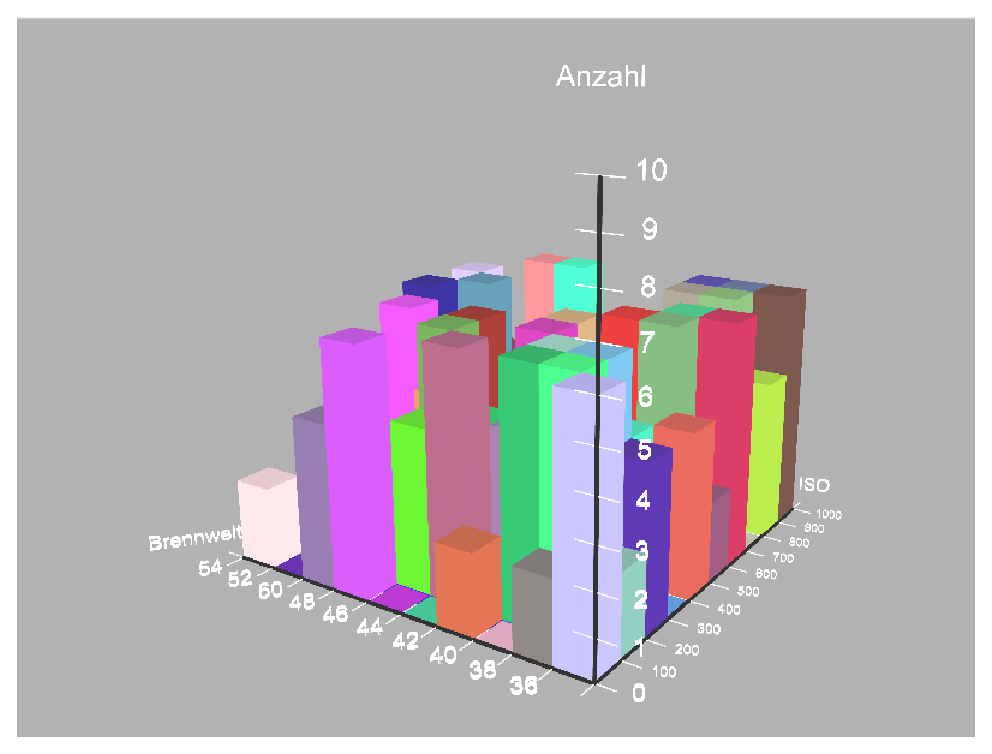
\includegraphics{images/3DHistogramm.eps}
						} 
						\caption{Ansicht eines 3D Histogramms}
						\label{diag:3dhistogramm}
					\end{minipage}  
				}    		
			\end{figure}
			Das Histogramm 3D erlaubt einen weiteren \gls{exif}-Paramter einer zweiten Achse, der z-Achse, zuzuweisen.
			Dabei wird die xz-Ebene in gleichgroße Rechtecke aufgeteilt. Die y-Achse gibt die Häufigkeit des zu betrachtenden Rechtecks an. Falls n Bildmengen mit der aktuellen Auswertung verbunden sind, so wird jedes Rechteck nochmals in n Rechtecke zerlegt ($ n \in \mathbb{N} $ und $ n>1 $). Das 3D Histogramm kann als \gls{jpg} exportiert werden.

		\item[/F340/] \textit{Boxplot:}\par 
			\begin{figure}[H]
				\centering
					\fbox{
						\begin{minipage}{13 cm}
							\centering
							% Generated with LaTeXDraw 2.0.2
% Tue Nov 17 17:46:01 CET 2009
% \usepackage[usenames,dvipsnames]{pstricks}
% \usepackage{epsfig}
% \usepackage{pst-grad} % For gradients
% \usepackage{pst-plot} % For axes
\scalebox{0.75} % Change this value to rescale the drawing.
{
\begin{pspicture}(0,-6.5467873)(9.0458,6.554775)
\definecolor{color812b}{rgb}{0.4980392156862745,0.6705882352941176,1.0}
\definecolor{color817b}{rgb}{0.9411764705882353,0.6941176470588235,0.08235294117647059}
\psframe[linewidth=0.07,dimen=outer,fillstyle=solid,fillcolor=color812b](3.6458,2.571025)(2.4458,-3.228975)
\psline[linewidth=0.07cm,tbarsize=0.07055555cm 5.0]{-|*}(3.0458,2.571025)(3.0458,4.671025)
\psline[linewidth=0.07cm,tbarsize=0.07055555cm 5.0]{|-}(3.0458,-5.228975)(3.0458,-3.228975)
\psline[linewidth=0.068cm,linecolor=red](2.5178,-1.428975)(3.5738,-1.428975)
\psdots[dotsize=0.204](3.0458,-0.628975)
\psframe[linewidth=0.07,dimen=outer,fillstyle=solid,fillcolor=color817b](7.6458,-0.028975)(6.4458,-3.528975)
\psline[linewidth=0.07cm,tbarsize=0.07055555cm 5.0]{-|*}(7.0458,-0.028975)(7.0458,2.071025)
\psline[linewidth=0.07cm,tbarsize=0.07055555cm 5.0]{|-}(7.0458,-4.716975)(7.0458,-3.514975)
\psline[linewidth=0.068cm,linecolor=red](6.5178,-1.428975)(7.5738,-1.428975)
\psdots[dotsize=0.204](7.0458,-1.228975)
\rput(1.0458,-5.728975){\psaxes[linewidth=0.04,labels=y,ticksize=0.1458cm,dx=1.0cm,dy=0.87cm,Dx=20,Dy=100]{->}(0,0)(0,0)(8,12)}
\usefont{T1}{ptm}{m}{n}
\rput(3.0208,-6.318975){Bildmenge 1}
\usefont{T1}{ptm}{m}{n}
\rput(7.0353312,-6.318975){Bildmenge 2}
\usefont{T1}{ptm}{m}{n}
\rput(0.42439374,6.381025){ISO}
\end{pspicture} 
}

							\caption{Ansicht eines Boxplots}
							\label{diag:boxblot}
						\end{minipage}  
					}    		
			\end{figure}


		\item[/F350/] \textit{Punktewolke:}\par		
			\begin{figure}[H]
				\centering
				\fbox{
					\begin{minipage}{13 cm}
						\centering
						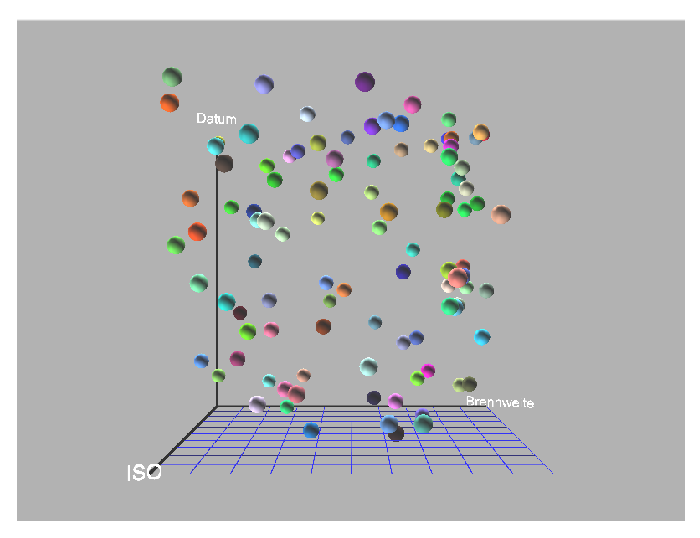
\includegraphics{images/punktewolke.eps} 
      			\caption{Ansicht einer Punktewolke}
      			\label{punktewolke}
					\end{minipage}  
    		}    		
			\end{figure}

	\end{description}

\subsection{Auswertungsmanagement}

\label{subsec:auswertungsmgmt}

	Eine Auswertung ist eine Verknüpfung von ein oder mehreren Bildmengen mit einem Diagrammtyp. Eine Auswertung ist dabei folgendermaßen definiert:

	\begin{itemize}

		\item Eine Auswertung kann auch ohne Auswahl ein oder mehrerer Bildmengen existieren. 

		\item Eine Auswertung hat einen frei definierbaren und vom Projektkontext abhängigen eindeutigen Namen, der zwischen einem und 200 Zeichen lang sein muss. Zu beachten ist, dass der Name automatisch um eine vorangestellte Zeichenkette ergänzt wird, die den Namen des gewählten Diagrammtyps beinhaltet.

		\item Eine Auswertung wird über eine interne ID eindeutig identifiziert.

	\end{itemize}

	% TODO Gui
	Wird ein Projekt geöffnet, werden alle in der Projektkonfigurationsdatei definierten Auswertungen \gls{lexgraph} sortiert angezeigt. Die erste Auswertung der Liste (falls vorhanden), wird dabei automatisch auf aktiv gesetzt (siehe Kapitel GUI).

	\begin{description}
		
		% TODO Formulierung
		\item[/F410/] \textit{Anlegen einer neuen Auswertung:}\par Durch betätigen der Schaltfläche "`Erstellen"' in dem Bereich "`Auswertungen"', wird ein Assistent gestartet, der den Benutzer durch die Auswertungserstellung führt.\par Über die Schaltfläche "`weiter"' kann der Benutzer dabei auf den nächsten Schritt wechseln, sofern er in der aktuellen Eingabemaske keine Fehleingabe getätigt hat. Durch betätigen der Schaltfläche "`zurück"', kann der Benutzer hingegen zu einem bereits getätigten Schritt wechseln. Auch hierbei wird vor dem Druck auf "`weiter"' überprüft, ob alle Eingabedaten immer noch korrekt sind.\par Folgende Schritte führt der Assistent aus:

			\begin{enumerate}

				\item \textbf{Diagrammtyp festlegen.}

					\begin{itemize}

						\item Festlegen eines Auswertungsnamens.

						\item Eine optionale Beschreibung der Auswertung.

						\item Auswahl eines Diagrammtyps (siehe Kapitel \ref{subsec:diagrammmgmt}).\par Bei der Auswahl, wird eine Livevorschau des Diagramms mit einem Dummydatensatz angezeigt, sowie eine kurze Beschreibung über Sinn und Zweck des Diagramms.\par Hier kann auch eine bereits in dem aktiven Projekt vorhandene Auswertung, als Vorlage verwendet werden. Dabei werden alle Werte der Auswertungsvorlage übernommen, bis auf die ID und der Name. Diese beiden Werte müssen neu generiert werden, damit die Definition nicht verletzt wird.

					\end{itemize}

				\item \textbf{Parameter festlegen}.\par Festlegen der X, Y oder Z Achse (je nach Diagrammtyp - siehe Kapitel \ref{subsec:diagrammmgmt}). Mit Festlegen ist hier das Verknüpfen mit \gls{exif}-Parametern gemeint. Optional kann eine Beschreibung angegeben werden, die dann anstatt der Bezeichnung des \gls{exif}-Parameters verwendet wird.

				\item \textbf{Bildmengen festlegen}.\par Hier werden Bildmengen des aktuell aktiven Projektes mit der Auswertung verknüpft. Außerdem kann hier anhand bestimmter \gls{exif}-Parametern eine Reduzierung der gesamten Bildmenge bewirkt werden (\textit{Filterung der Daten}).

			\end{enumerate}

			Nach Beendigung des Assistenten, wird die Auswertung gespeichert und, falls bereits Bildmengen mit der Auswertung verknüpft wurden, geöffnet.
		
		\item[/F420/] \textit{Aktivieren einer Auswertung:}\par Um eine Auswertung zu aktivieren, muss man sie in der Liste der Auswertungen, im Bereich "`Auswertungen"', auswählen.
		
		\item[/F430/] \textit{Bearbeiten einer Auswertung:}\par Um eine Auswertung zu bearbeiten, muss sie aktiv sein. Durch betätigen der Schaltfläche Bearbeiten"' in dem Bereich "`Auswertungen"', wird ein Dialog geöffnet, der die gleichen Auswahlmöglichkeiten des Assistenten aus \textbf{/F310/} enthält. Diese sind über Tabs auswählbar und sind mit den Werten der Auswertung vorbelegt. Nach dem Beenden des Dialogs, wird die Auswertung automatisch gespeichert.
				
		\item[/F440/] \textit{Entfernen einer Auswertung:}\par Um eine Auswertung zu entfernen, muss sie aktiv sein. Durch betätigen der Schaltfläche Entfernen"' in dem Bereich "`Auswertungen"', werden folgende Aktionen ausgelöst:

			\begin{enumerate}

				\item Es wird eine Sicherheitsabfrage (ein Dialog mit Ja/Nein Auswahlmöglichkeit) angezeigt, die dem Benutzer die Möglichkeit gibt, das Entfernen abzubrechen.

				\item Die Auswertung wird aus der Liste der Auswertungen entfernt.

				\item Dem Benutzer wird eine Rückmeldung gegeben, ob das Entfernen erfolgreich war oder ob es einen Fehler gab.

				\item Nach dem Entfernen, ist die erste Auswertung (falls vorhanden) in der Liste aktiv.

			\end{enumerate}
			
	\end{description}

\subsection{Exif-Auswertung}

	\begin{description}

		% TODO XXX->Ref
		\item[/F510/] \textit{Extraktion von \gls{exif} Daten:}\par Beim Einlesen von Bildern im \gls{jpg}-Format, werden nur die \gls{exif}-Parameter eingelesen, nicht die Bilddaten. Die \gls{exif}-Parameter, die verarbeitet werden, sind unter XXX definiert. Die Daten werden nur während der Programmausführung intern gespeichert, dies hat zur konsequenz, dass bei jedem Programmstart, alle \gls{exif}-Parameter neu eingelesen werden müssen (siehe Kapitel \ref{subsec:projektmanagement} \textbf{/F130/}).
	
	\end{description}